\subsection{Android application}
\chapterauthor{Theolin, Henrik (no one)}
The main reason for this project is to give a sailor qualitative feedback and help in clearing the mind of the techniques required to achieve a smooth sailing experience so that the sailor can focus on the joy of sailing. It is therefore crucial that the data is displayed in a manner that is easy to interpret and provide the help that is called for. To increase the flexibility of the design it was decided to implement several different user interfaces that the user could switch between while running the application. This was determined to be a good way of increasing the chances that the user would find a interface to it's liking. It was also determined that not only visual representaion would be the best way to go since the sailor needs to be in constant motion to counteract the forces applied on the ship by the wind and current. This would make watching a screen to retreive information somewhat difficult. Other ways of representing data was implemented using text-to-speech where the sailor would get important information by sound aswell as text. Vibration was also used with different vibration sequences depending on diffenrent sates of the ship.


\subsubsection{Feedback}
For the feedback states used in the application there were some approximations and simplifications made for easier implementation. A sailor can 
\subsubsection{Visual Feedback}
It was determined that the visual feedback given to the sailor was to include very little text information and would consist mainly of images that changes position based on sensor data to give a good representation of what was going on with the ship. Because of different personal preferences the ability to switch between different layouts was implemented. To switch between different layouts a simple swipe on the screen toggled the view to the next layout. All layouts consisted of a subset of views from the complete set including
\begin{labeling}{alligator}
\item [\ref{feedback-incline} Incline]  displayed a ships relative incline against and artificial horizont
\item [\ref{feedback-pressure} Pressure] moved a pin along a colored bar to represent high of low pressure applied on the centerboard
\item [\ref{feedback-compass} Bearing] rotated a compass to show the ship relative bearing against true north
\item [\ref{feedback-map} Map] displayed current location of the ship
\item [\ref{feedback-drift} Drift] was represented with a colored bar with two arrows that moved to the relative drift direction to show the sailor if the ship was holding it's set navigaitional reference.
\item [Feedback] a text that changed values based on the current state of the boat
\item [Height] the height of the centerboard was represented with a visual centerboard moving up and down along a graphical ruler
\item [Wave frequency] displayed a wave moving towards a ship at a speed representing different periods of the waves.
\end{labeling}

\begin{figure}[H]
\centering
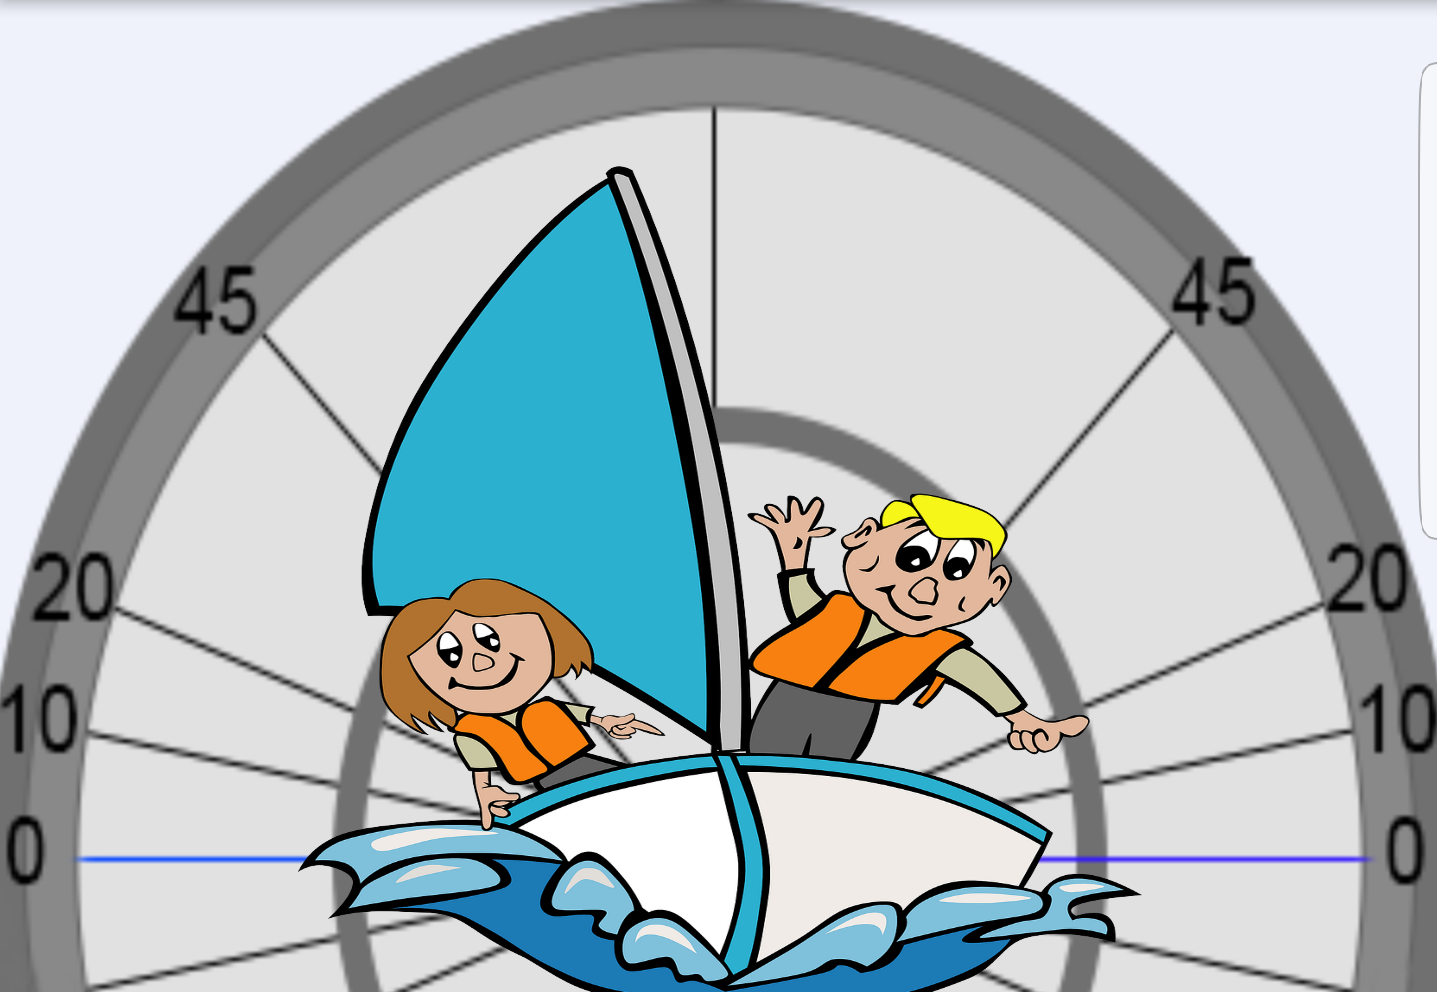
\includegraphics[width=0.6\textwidth]{Figures/incline.png}
\caption{Incline feedback view}
\label{feedback-incline}
\end{figure}
\begin{figure}[H]
\centering
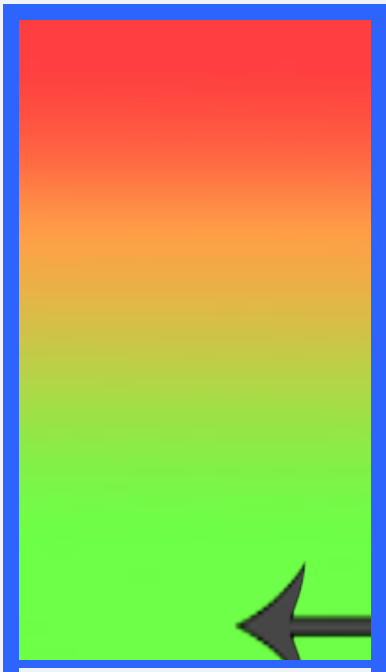
\includegraphics[width=0.3\textwidth]{Figures/pressure.png}
\caption{Pressure feedback view}
\label{feedback-pressure}
\end{figure}
\begin{figure}[H]
\centering
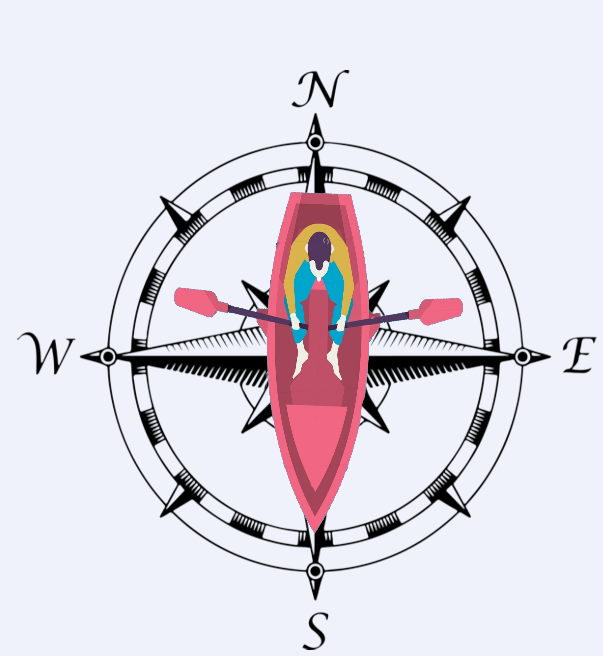
\includegraphics[width=0.6\textwidth]{Figures/compass.png}
\caption{Bearing feedback view}
\label{feedback-compass}
\end{figure}
\begin{figure}[H]
\centering
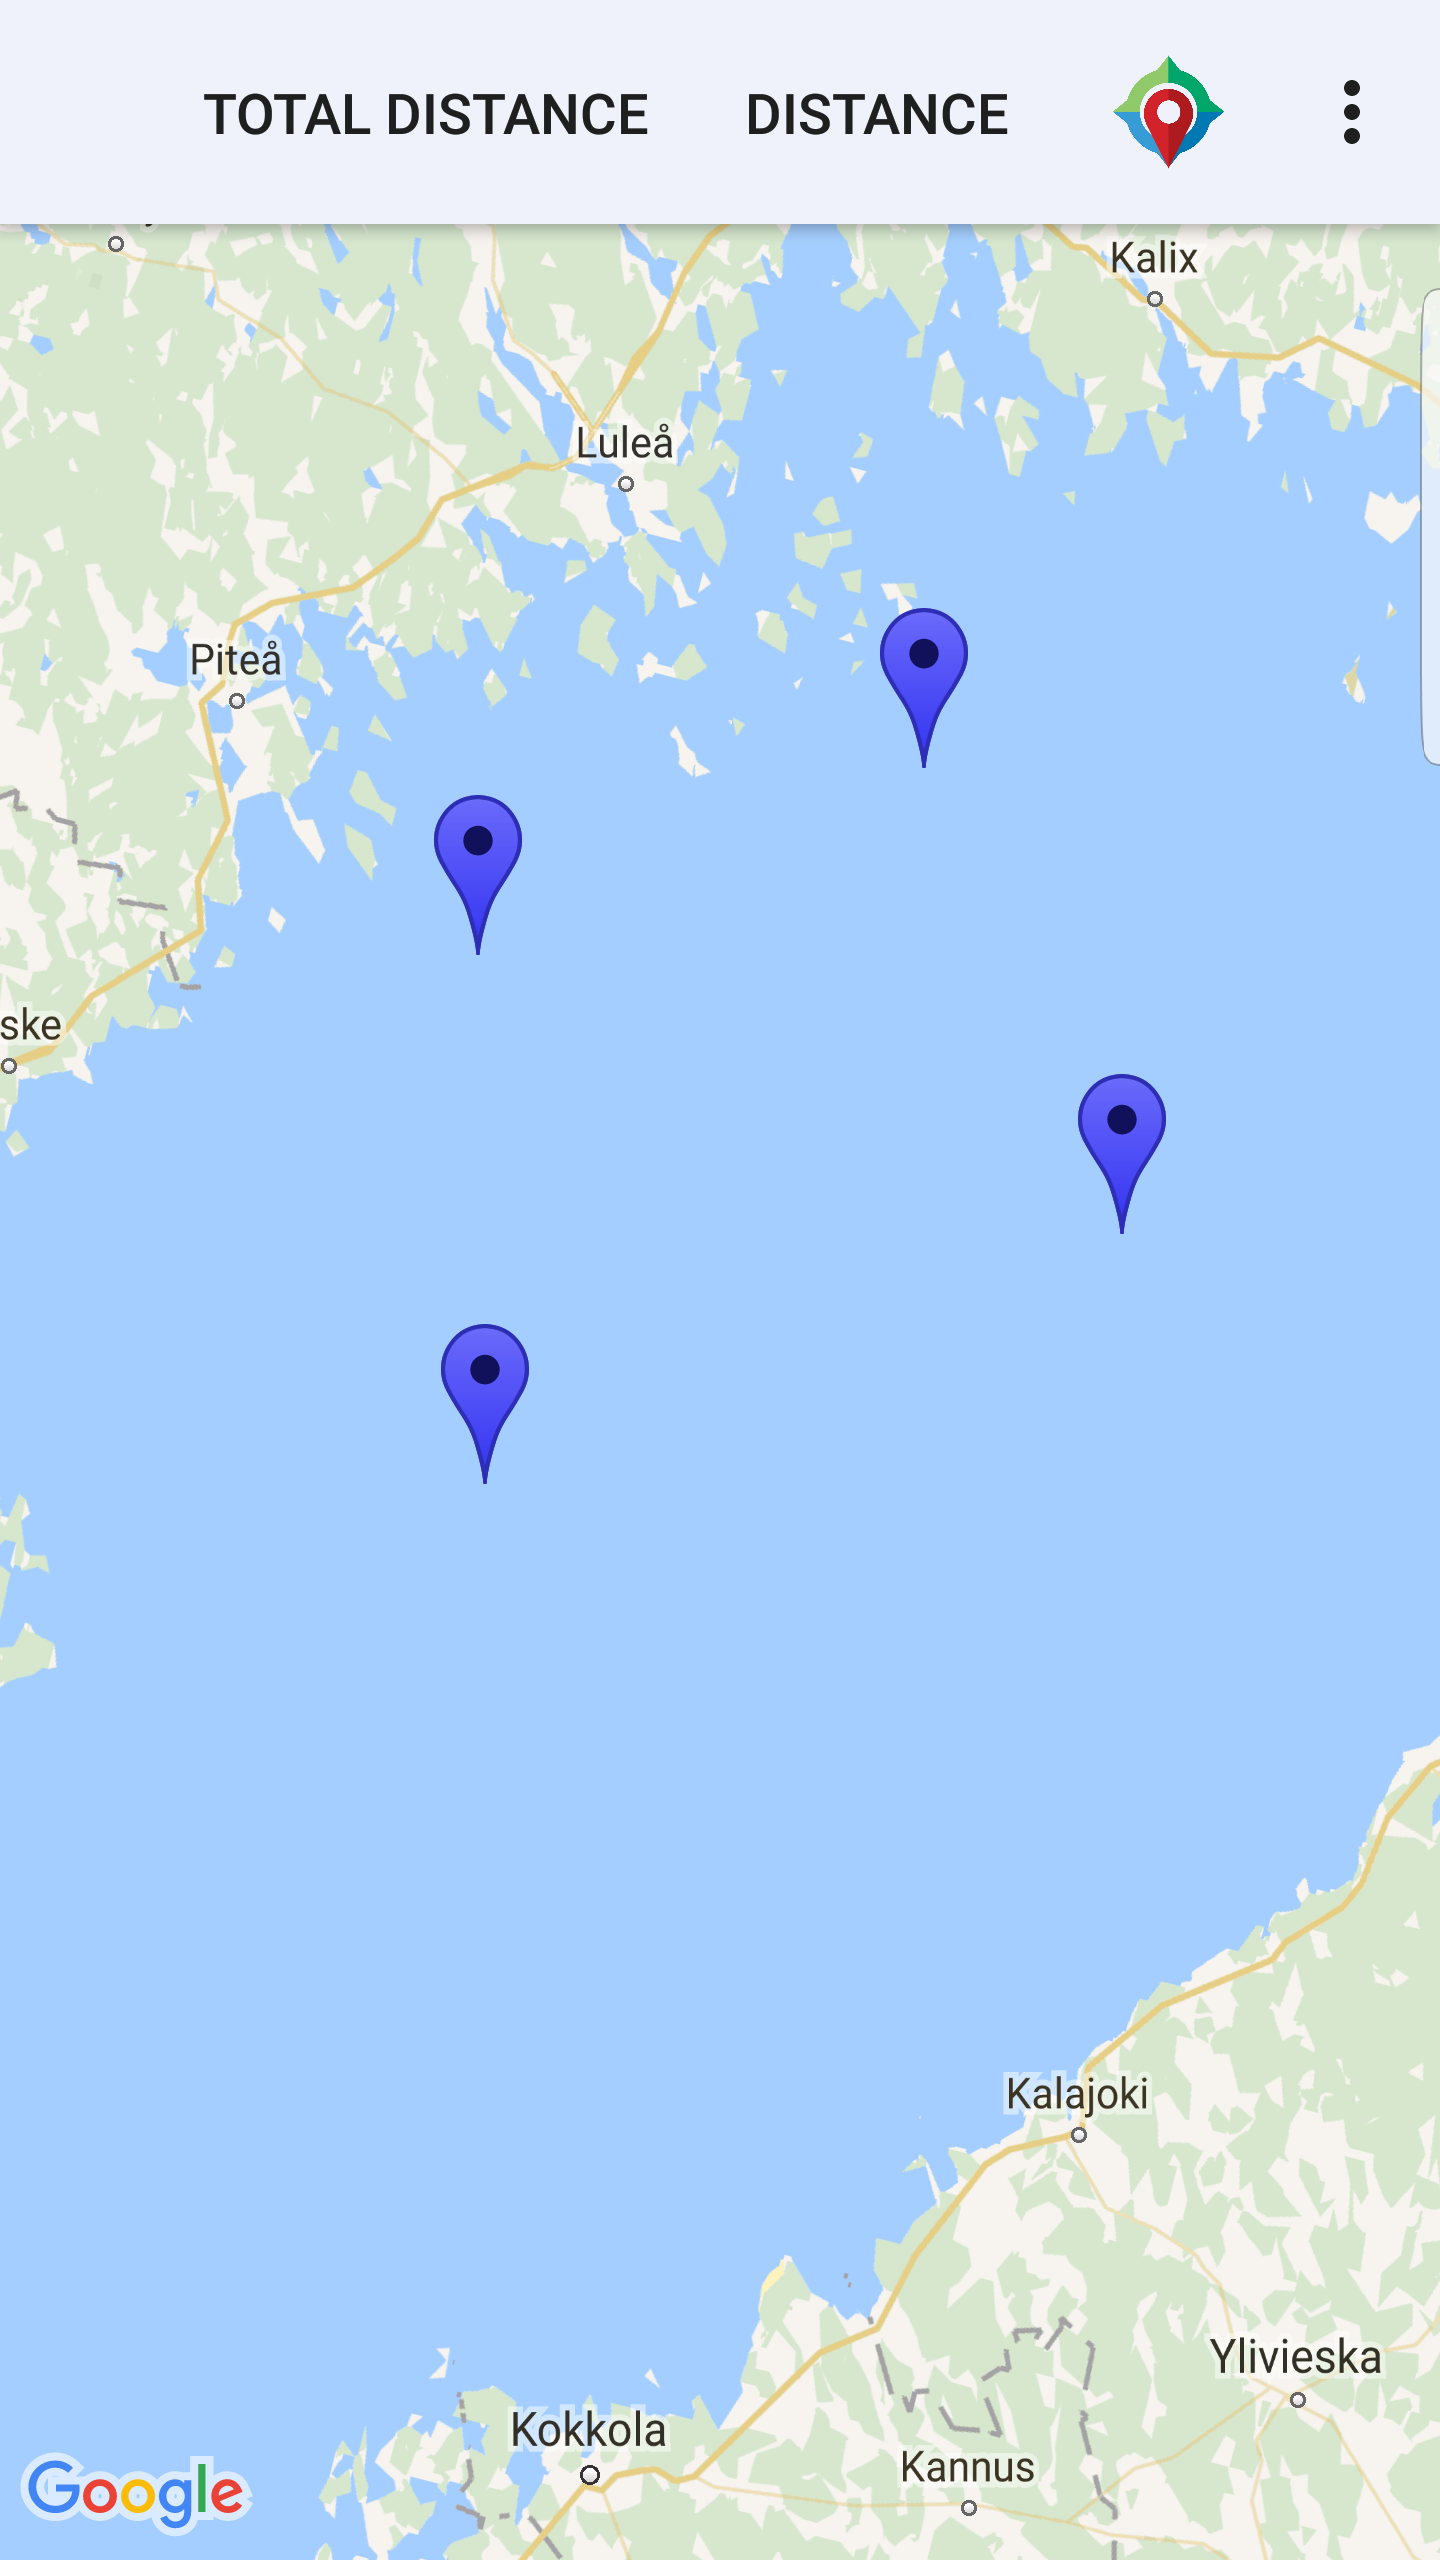
\includegraphics[width=0.4\textwidth]{Figures/map.png}
\caption{Map feedback view}
\label{feedback-map}
\end{figure}
\begin{figure}[H]
\centering
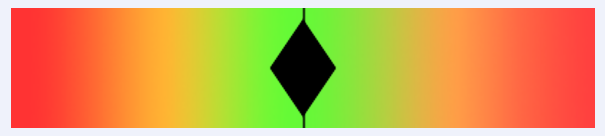
\includegraphics[width=0.6\textwidth]{Figures/drift.png}
\caption{Drift feedback view}
\label{feedback-drift}
\end{figure}
The figures were chosen at a development stage and improvements can easily be made by adding different \textit{PNG} files in android studio.

\subsubsection{Audio feedback}
Based on values from the sensors different states were implemented and for each state a text was read out to the sailor. A priority for each state to prevent less important events from interrupting the more important ones. The feedback was implemented such that the audio feedback would continue even if the device was put in sleep mode.

\subsubsection{Haptic feedback}
Based on the same states as the audio feedback vibration was also implemented. The frequency and length of the vibrations were implemented in such a way the each state had a unique signature that could be recognised by the sailor after some practise with the system.

\subsubsection{Log}
The ability to analyse the sailtrip was determined an important feature for the user so a log was implemented and stored on the device internal storage. These files could then be read or deleted at a later date. Storing a log was implemented such that the sailor would need to start a logging session after bluetooth connection had been established to the ship. After the log was started it would create a file on the device internal storage and write sensor data to the file at the same frequency as the data was transmitted by the system. While logging was active the device would continue to store information even if the screen was put in sleep mode so that the sailor could choose to only log data and not view the information displayed on the screen. After the sailtrip was finished the sailor could read the saved log file and receive a summary of the trip \ref{log-summary}. More information from the log could be analysed by reading graphs \ref{log-graph} where the sensor data was shown with respect to time.

\begin{figure}[H]
\centering
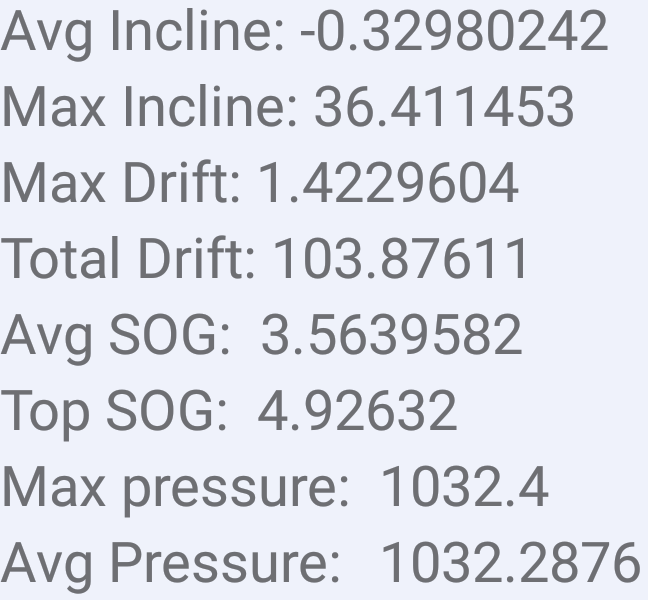
\includegraphics[width=0.4\textwidth]{Figures/log_data.png}
\caption{Log data summary}
\label{log-summary}
\end{figure}

\begin{figure}[H]
\centering
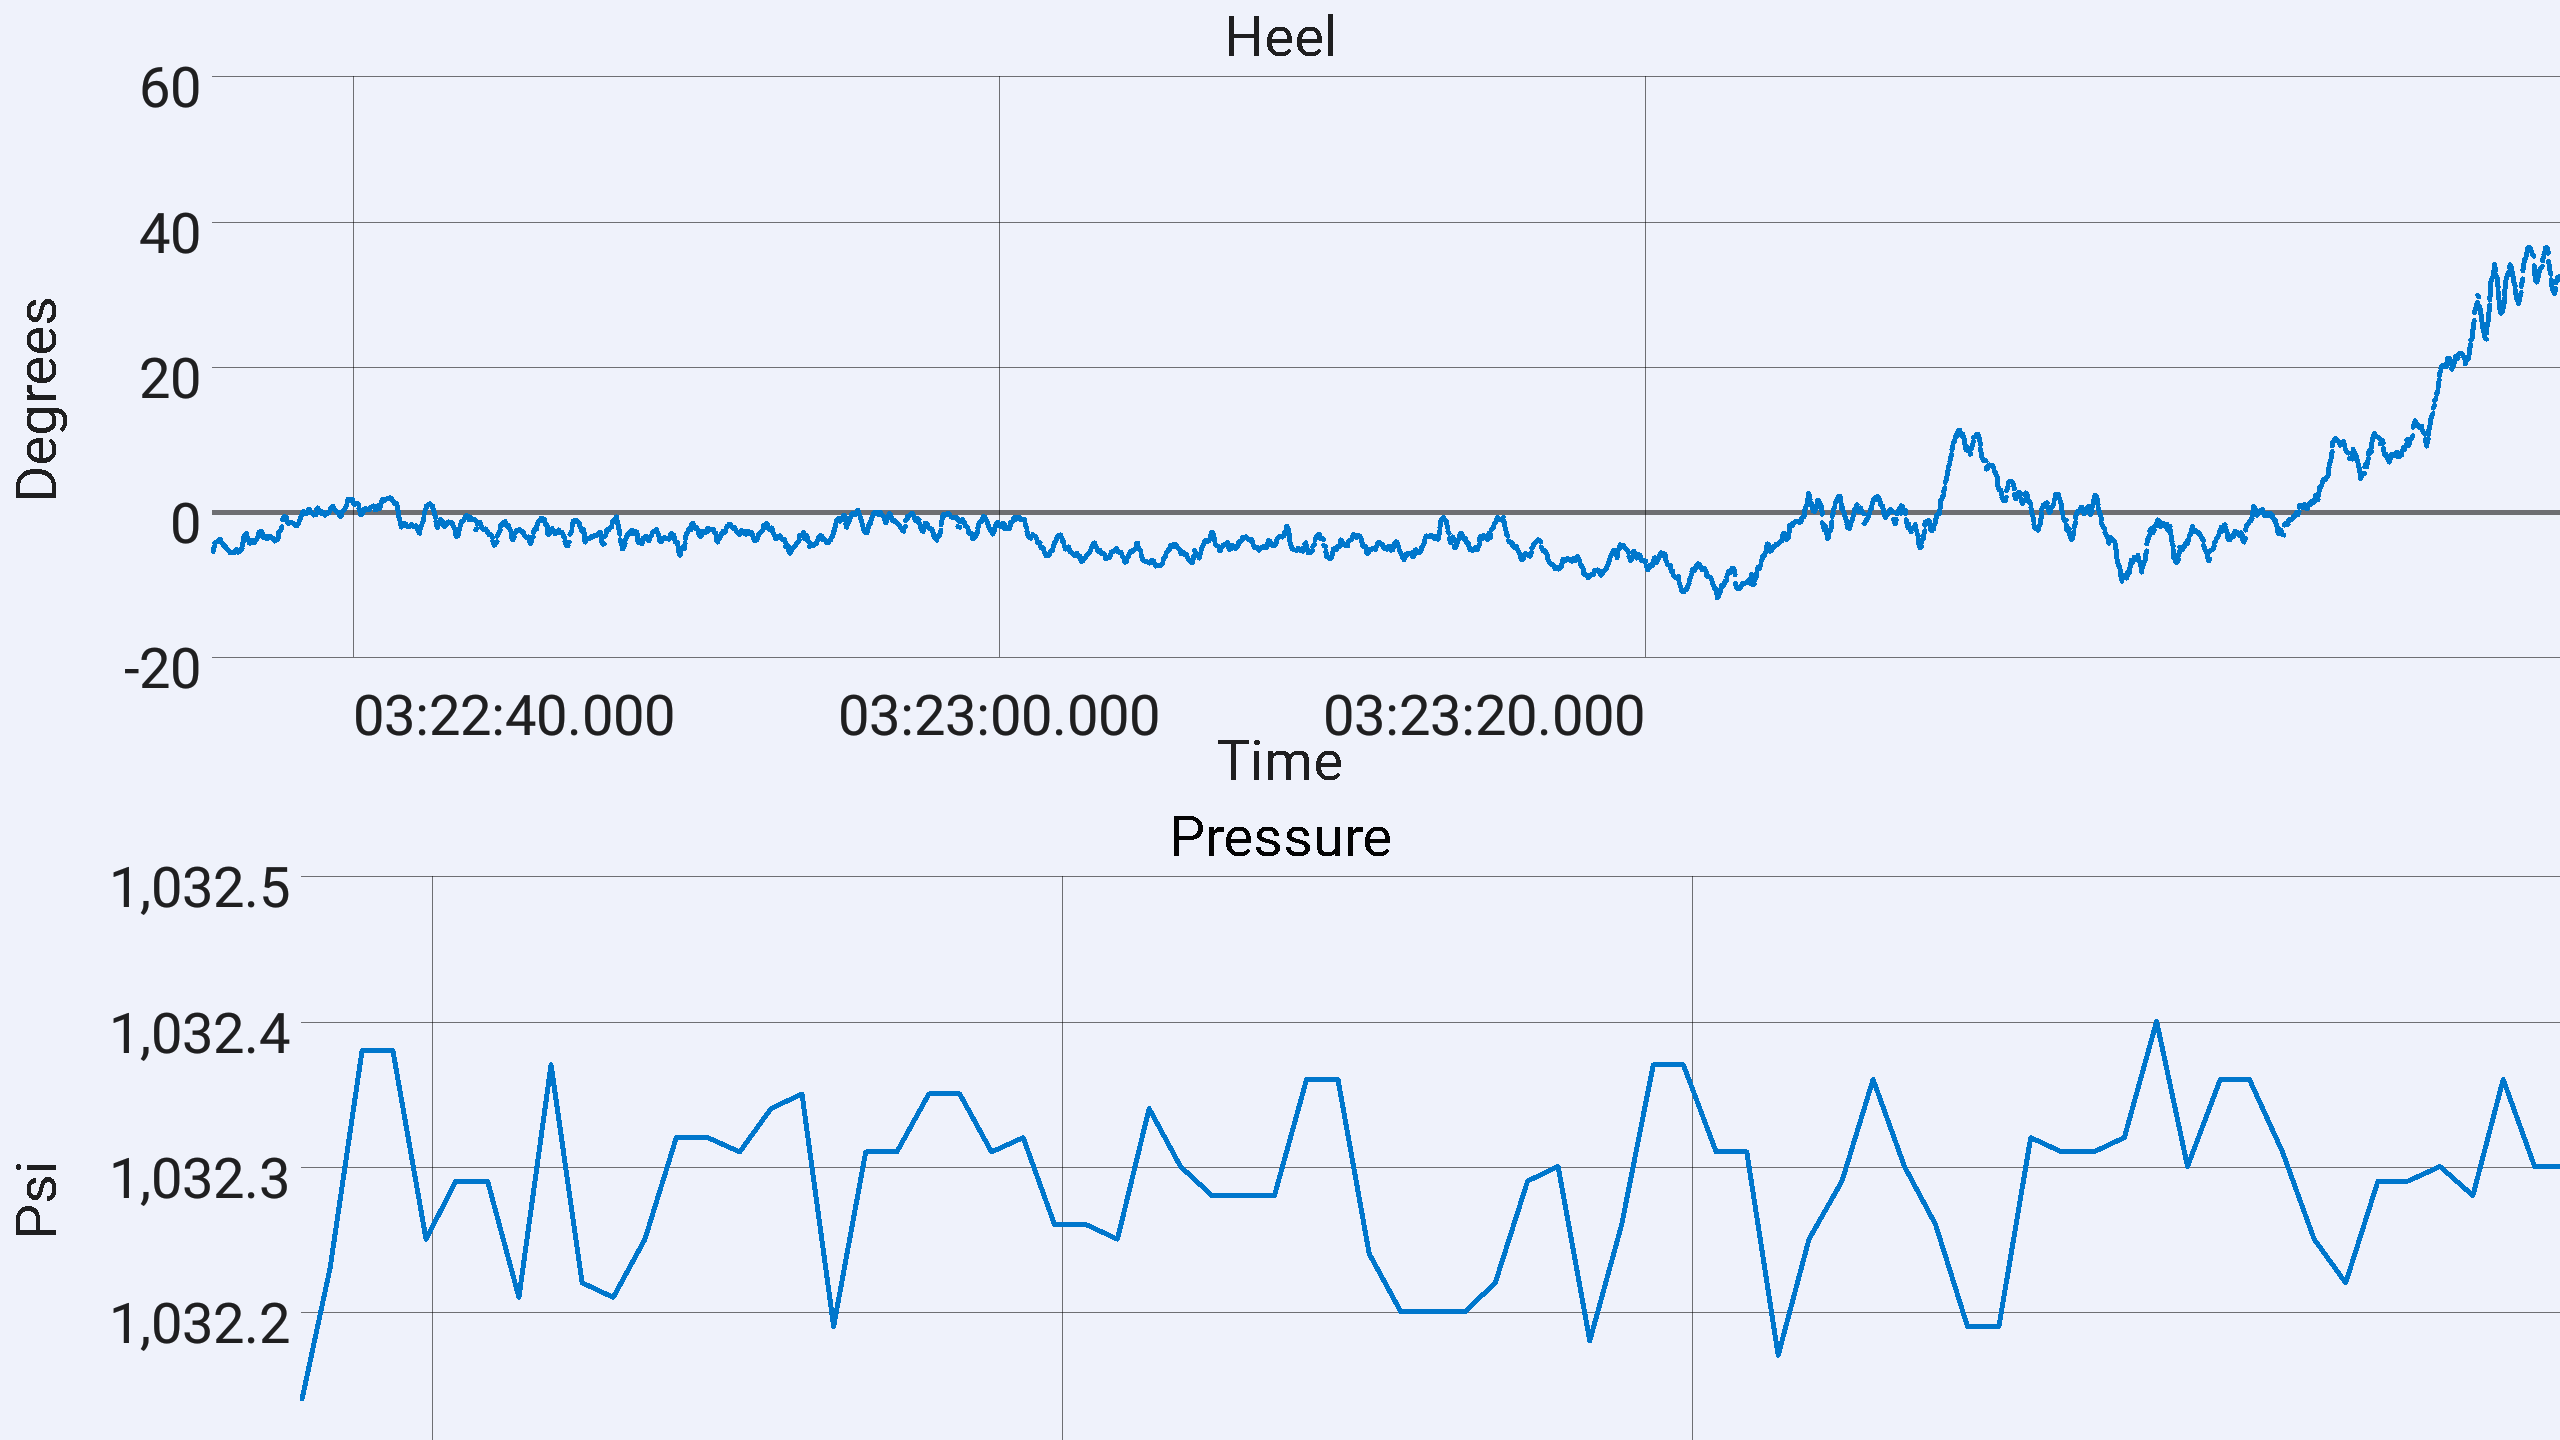
\includegraphics[width=0.7\textwidth]{Figures/log_graph.png}
\caption{Log graphs}
\label{log-graph}
\end{figure}

\subsubsection{Bluethooth connection}
A list of all devices in the nearby area was displayed when the user decided to connect to the system, this added flexibility to the user and allowed connection between multiple systems with different MAC-adressess. The application uses bluetooth low energy technology to match the systems implementation. This allowed for the device to recieve notifications when the data is altered on the system and updates would occur in different frequencies for different types of data. To ensure a stable connection between the system and the device the connection class was implemented as an android service\cite{android-service}. This allowed the device to keep the connection alive between different views and even when the device was put to sleep mode.

\subsubsection{Map}
For the sailor to get more information about location a map was implemented. The sailor then had the ability to see a path over the trip and the total distance traveled. Waypoint could be placed if the sailor wanted to decide in advance a certain trip. The distance of all the waypoints was displayed and the distance currently traveled to give the sailor information on how long the trip was and how much of the trip was left to be sailed. A path to the nearest waypoint was showed to the sailor to help navigating, when the sailor way close to the waypoint the path to the next waypoint was shown.

\subsubsection{Drift}
Calculation of leeward drift was done by inspection of both pressure produced on the centerboard and by calculating the distance from an estimated destination point with the position received from the \textit{GPS}. By using the \textit{GPS} position and the ships bearing from the systems magnetometer a \textit{rhumb line}\cite{rhumb-line} was derived and the new estimated position was calculed with
%δ = d/R	(angular distance)
%φ2 = φ1 + δ ⋅ cos θ	
%Δψ = ln( tan(π/4 + φ2/2) / tan(π/4 + φ1/2) )	(‘projected’ latitude difference)
%q = Δφ/Δψ (or cos φ for E-W line)	
%Δλ = δ ⋅ sin θ / q	
%λ2 = λ1 + Δλ
\begin{align*}
  &\begin{aligned}
  \delta &= d/R 
  \end{aligned}\\
 &\begin{aligned}
  \varphi_2 &= \varphi_1 + \delta \cdot \cos{\theta}
  \end{aligned}\\
 &\begin{aligned}
  \Delta\psi = \ln { \bigg( \tan{\frac{n}{4} + \frac{\varphi_2}{2}} \bigg/ \tan{\frac{n}{4} + \frac{\varphi_1}{2}} \bigg)}
  \end{aligned}\\
 &\begin{aligned}
  q = \frac{\Delta\varphi}{\Delta\varphi}
  \end{aligned}\\
 &\begin{aligned}
  \Delta\lambda = \delta\cdot\sin\frac{\theta}{q}
  \end{aligned}\\
 &\begin{aligned}
  \lambda_2 = \Delta\lambda_1 + \Delta\lambda
  \end{aligned}\\
\end{align*}
where $R$ is the earths radius, $d$ is the distance traveled, $\theta$ is ships bearing, $\lambda_1$ and $\psi_1$ is the point of origin in longitude and latitude. This new estimated position was then compared to the next positional data from the \textit{GPS} and the distance between these points was caluculated using \textit{Equirectangular projection}\cite{equitriangular}
%x = Δλ ⋅ cos φm
%y = Δφ
%d = R ⋅ √x² + y²
\begin{align*}
  &\begin{aligned}
  x = \Delta\lambda \cdot \cos\frac{\Delta\varphi}{2}
  \end{aligned}\\
 &\begin{aligned}
  y = \Delta\varphi
  \end{aligned}\\
 &\begin{aligned}
  d = R\cdot\sqrt{x^2+y^2}
  \end{aligned}\\
\end{align*}
where $\Delta\lambda$ and $\Delta\varphi$ are the differences in longitude and latitude for two location points. This function had high performace gain but was less accurate over large distances then for example the \textit{Haversine formula}\cite{haversine}. Since for this function only small changes in distance were calculated the accuracy was more then adequate. A problem with this way of calculating leeward drift is the accuracy of the \textit{GPS} readings. This could be improved with filtering.


























